%(BEGIN_QUESTION)
% Copyright 2009, Tony R. Kuphaldt, released under the Creative Commons Attribution License (v 1.0)
% This means you may do almost anything with this work of mine, so long as you give me proper credit

Determine the proper control action ({\it direct} or {\it reverse}) for the controller in this pH neutralization system, assuming direct action on the part of the transmitter (i.e. increasing pH = increasing mA signal) and an air-to-open (ATO) control valve:

$$\includegraphics[width=15.5cm]{i04137x01.eps}$$

\vskip 20pt \vbox{\hrule \hbox{\strut \vrule{} {\bf Suggestions for Socratic discussion} \vrule} \hrule}

\begin{itemize}
\item{} If the pH transmitter in this control system were mis-calibrated so that it always registered 0.5 pH units too high, how would this affect the real pH value of the treated water?
\item{} If the control valve in this control system were mis-calibrated so that it always opened up 7\% more than it was supposed to, how would this affect the real pH value of the treated water?
\item{} If the controller were configured for the wrong action (e.g. direct instead of reverse, or vice-versa), what would likely be the result in this process?
\item{} If the neutralizing reagant were switched from acid to caustic, would this require a change in the controller's action?  Why or why not?
\item{} Will changes in acid density affect the accuracy of the acid flowmeter?  Why or why not?
\item{} If the water temperature happens to increase but there is no RTD in the pH probe to compensate for temperature changes, will the pH transmitter register too high, too low, or will the change be impossible to predict?
\item{} Is the influent water {\it acidic} or {\it alkaline}, based on this neutralization system design?
\end{itemize}

\underbar{file i04137}
%(END_QUESTION)





%(BEGIN_ANSWER)


%(END_ANSWER)





%(BEGIN_NOTES)

As pH rises (becomes more caustic), the AIC receives a higher 4-20 mA signal from the AT at the bottom of the mixing vessel.  In response, the AIC needs to add more acid to bring the pH back down to setpoint.  Since the acid control valve is air-to-open, this means the AIC must output a greater 4-20 mA signal to the valve.  Therefore, the controller needs to be configured for {\it direct} action.







\vskip 20pt \vbox{\hrule \hbox{\strut \vrule{} {\bf Virtual Troubleshooting} \vrule} \hrule}

This question is a good candidate for a ``Virtual Troubleshooting'' exercise.  Presenting the diagram to students, you first imagine in your own mind a particular fault in the system.  Then, you present one or more symptoms of that fault (something noticeable by an operator or other user of the system).  Students then propose various diagnostic tests to perform on this system to identify the nature and location of the fault, as though they were technicians trying to troubleshoot the problem.  Your job is to tell them what the result(s) would be for each of the proposed diagnostic tests, documenting those results where all the students can see.

During and after the exercise, it is good to ask students follow-up questions such as:

\begin{itemize}
\item{} What does the result of the last diagnostic test tell you about the fault?
\item{} Suppose the results of the last diagnostic test were different.  What then would that result tell you about the fault?
\item{} Is the last diagnostic test the best one we could do?
\item{} What would be the ideal order of tests, to diagnose the problem in as few steps as possible?
\end{itemize}

%INDEX% Chemistry, pH: neutralization
%INDEX% Process: water pH neutralization (generic)

%(END_NOTES)


